\chapter{Background}
\label{sec:background}

Test

\begin{figure}[ht]
	\begin{center}
		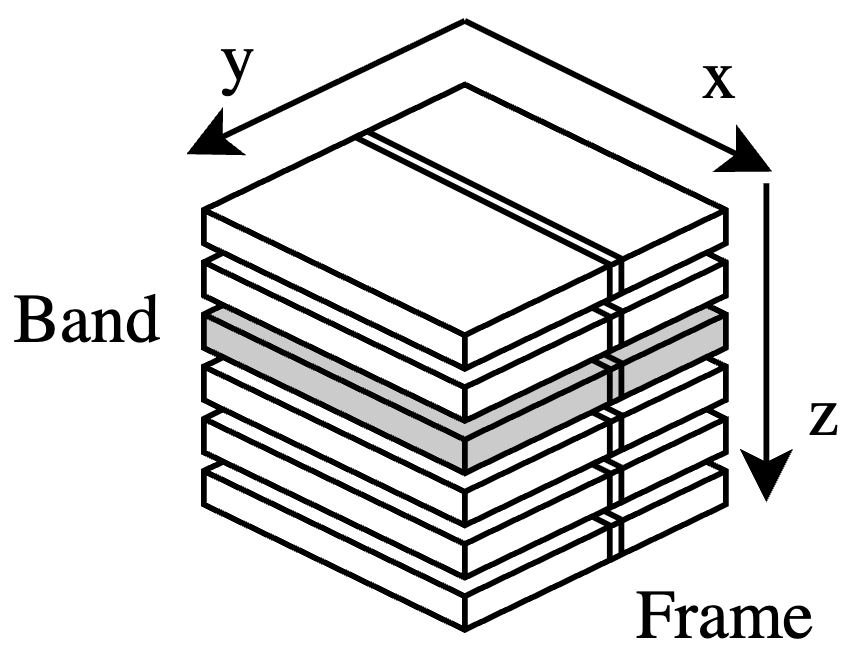
\includegraphics[width=0.3\textwidth]{figures/hsi.png}
	\end{center}
	\caption{}
	\label{fig:hsi}
\end{figure}

\newpage
of

\begin{figure}[ht]
	\begin{center}
		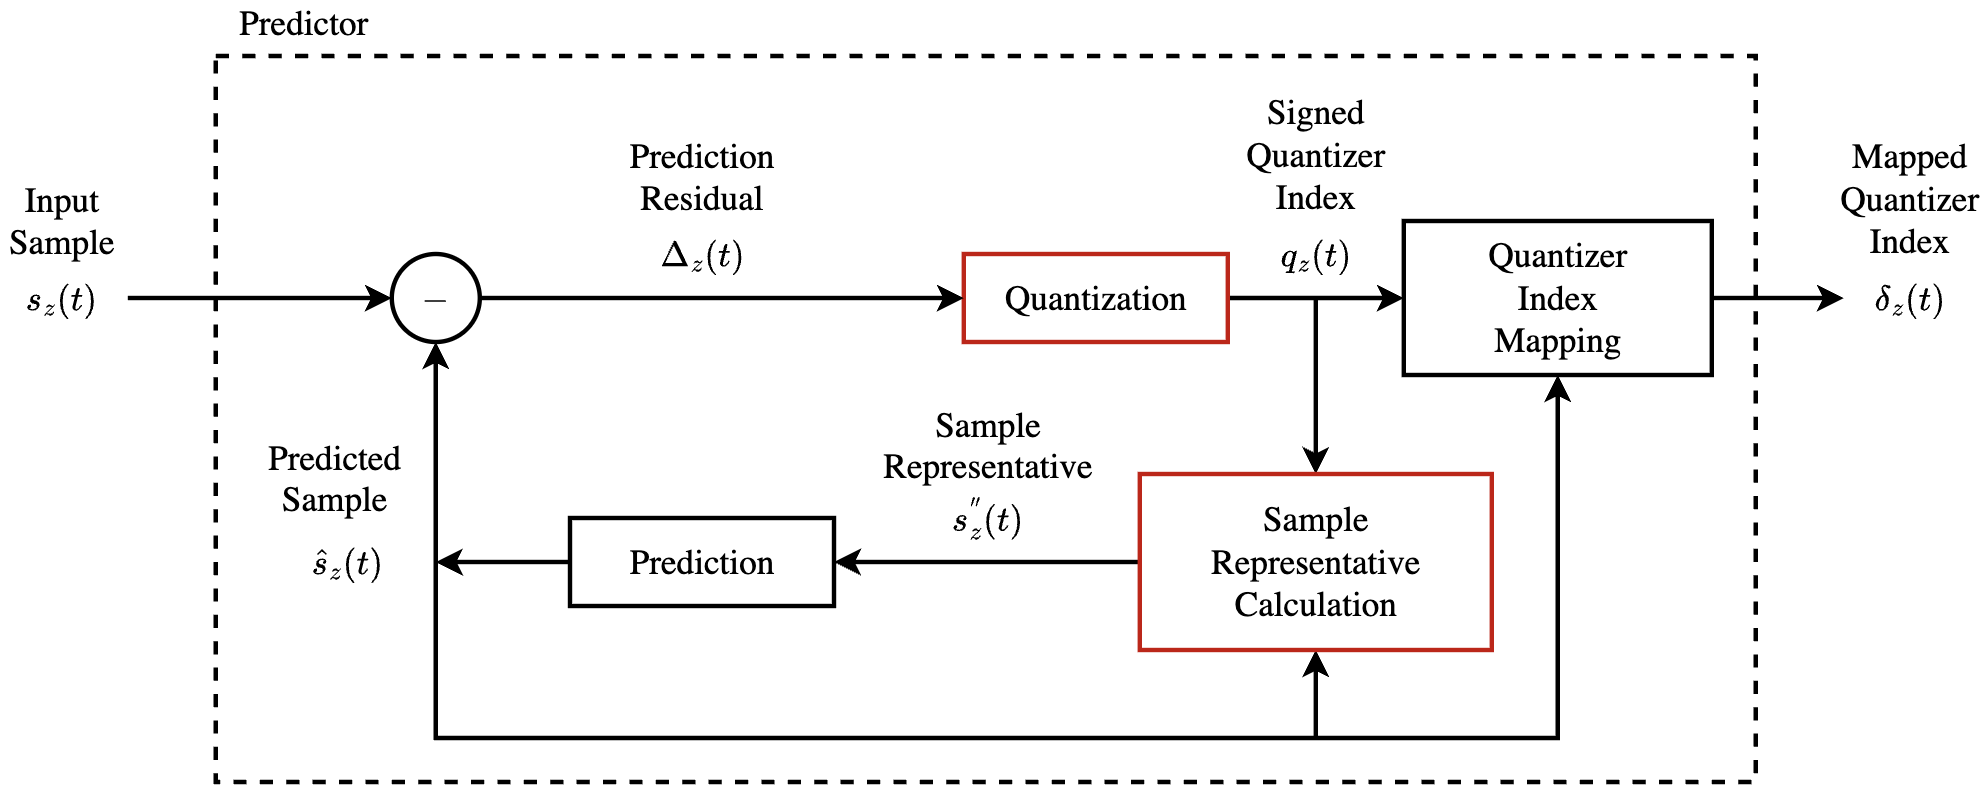
\includegraphics[width=0.9\textwidth]{figures/predictor-block.png}
	\end{center}
	\caption{}
	\label{fig:predictor-block}
\end{figure}

\newpage
multipage

\begin{figure}[ht]
	\begin{center}
		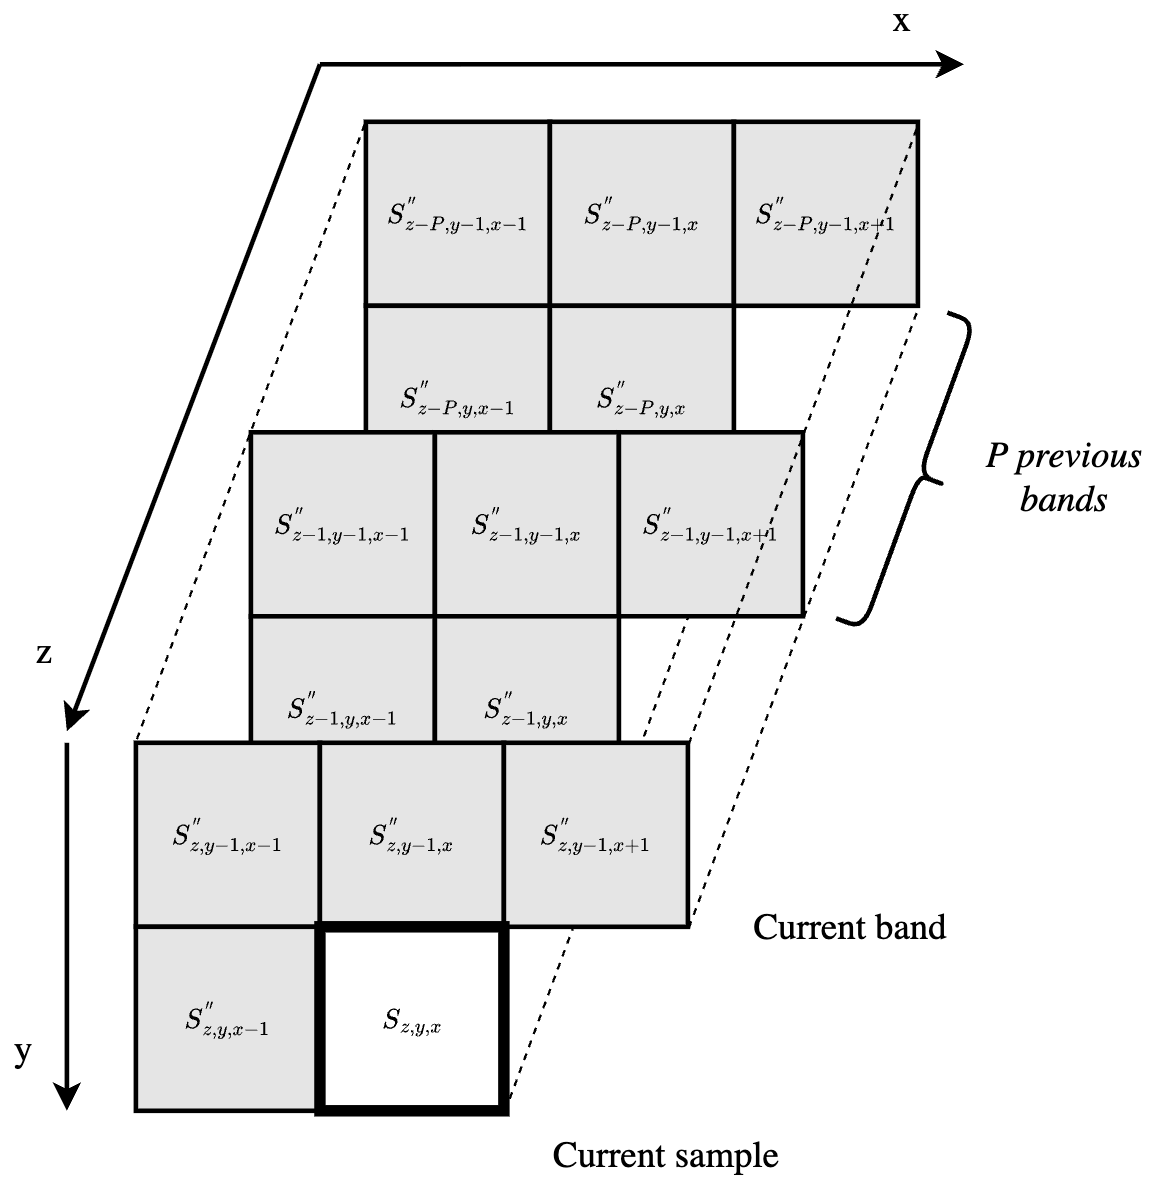
\includegraphics[width=0.7\textwidth]{figures/prediction-neighborhood.png}
	\end{center}
	\caption{}
	\label{fig:prediction-neighborhood}
\end{figure}

\begin{figure}[ht]
	\begin{center}
		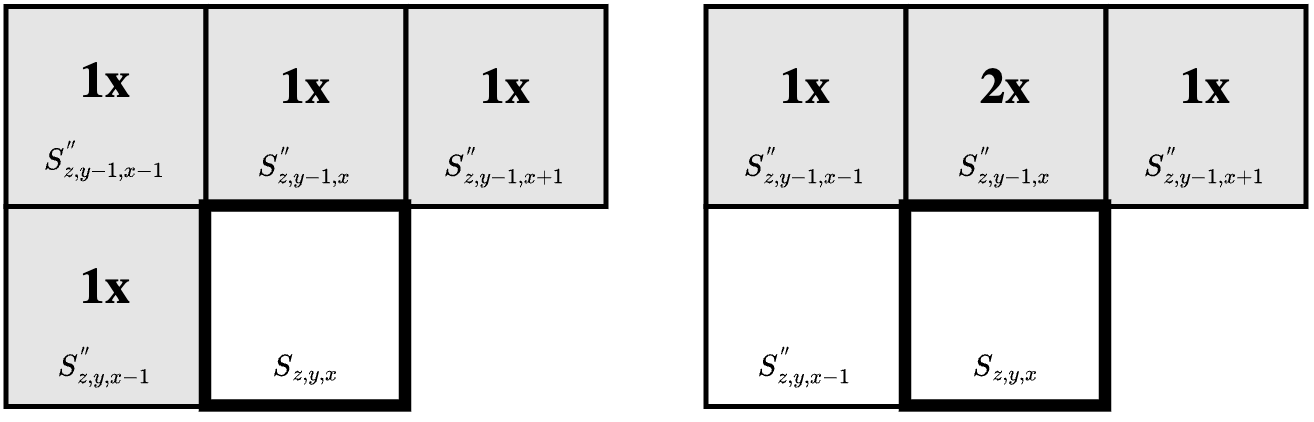
\includegraphics[width=0.7\textwidth]{figures/local-sums.png}
	\end{center}
	\caption{}
	\label{fig:local-sums}
\end{figure}

\begin{equation}
	\sigma_{z,y,x} =
	\begin{cases}
		s''_{z,\,y-1,\,x-1} + 2 s''_{z,\,y-1,\,x} + s''_{z,\,y-1,\,x+1},
		 & y > 0,\ 0 < x < N_X - 1,
		\\[6pt]
		4 s''_{z-1,\,y,\,x-1},
		 & y = 0,\ x > 0,\ z > 0,
		\\[6pt]
		2\!\left( s''_{z,\,y-1,\,x} + s''_{z,\,y-1,\,x+1} \right),
		 & y > 0,\ x = 0,
		\\[6pt]
		2\!\left( s''_{z,\,y-1,\,x-1} + s''_{z,\,y-1,\,x} \right),
		 & y > 0,\ x = N_X - 1,
		\\[6pt]
		4 s_{\text{mid}},
		 & y = 0,\ x = 0,\ z = 0.
	\end{cases}
	\label{eq:}
\end{equation}

\begin{equation}
	\mathbf{U}_z(t) =
	\begin{bmatrix}
		d_{z-1}(t)     \\
		d_{z-2}(t)     \\
		\vdots         \\
		d_{z-P^*_z}(t) \\
	\end{bmatrix},
	\label{eq:local-differences}
\end{equation}

\begin{equation}
	P^*_z = \min(z, P),
	\label{eq:prediction-bands}
\end{equation}

\begin{equation}
	\hat{d}_z(t) = \mathbf{W}_z(t) \cdot \mathbf{U}_z(t).
	\label{eq:predicted-central-local-difference}
\end{equation}

\begin{equation}
	\mathbf{W}_z(t)=
	\begin{bmatrix}
		\omega_z^{(1)}(t) \\
		\omega_z^{(2)}(t) \\
		\vdots            \\
		\omega_z^{(P^*_z)}(t)
	\end{bmatrix},
	\label{eq:weight-vector}
\end{equation}

\begin{equation}
	\omega_z^{(1)}(1) = \frac{7}{8} 2^{\Omega}, \qquad
	\omega_z^{(i)}(1) = \left\lfloor \frac{1}{8}\, \omega_z^{(i-1)}(1) \right\rfloor,
	\quad i = 2,3,\ldots,P_z^{*},
	\label{eq:weight-init}
\end{equation}

\begin{equation}
	\omega_{\mathrm{min}} = -2^{\Omega+2}, \: \omega_{\mathrm{max}} = -2^{\Omega+2} - 1.
	\label{eq:weight-min-max}
\end{equation}

\begin{equation}
	\omega^{(i)}_{z, \text{offset}}(t) = \left\lfloor \frac{1}{2} \left(2^{-\rho(t)} \cdot d_{z-i}(t) \cdot \text{sgn}^+[e_z(t)] + 1 \right) \right\rfloor,
	\label{eq:weight-offset}
\end{equation}

\begin{equation}
	e_z(t) = 2s'_z(t) - \tilde{s}_z(t).
	\label{eq:double-resolution-prediction-error}
\end{equation}

\begin{equation}
	\rho(t) = \operatorname{clip}\!\left(
	\nu_{\min} +
	\left\lfloor \frac{t - N_x}{t_{\mathrm{inc}}} \right\rfloor,
	\{ \nu_{\min}, \nu_{\max} \}
	\right)
	+ D - \Omega,
	\label{eq:weight-update-scaling-exponent}
\end{equation}

\begin{equation}
	\omega^{(i)}_z(t + 1) = \text{clip} \left( \omega^{(i)}_z(t) + \omega^{(i)}_{z, \text{offset}}(t), \{ \omega_{min}, \omega_{max} \} \right),
	\label{eq:weight-update}
\end{equation}


\begin{figure}[ht]
	\begin{center}
		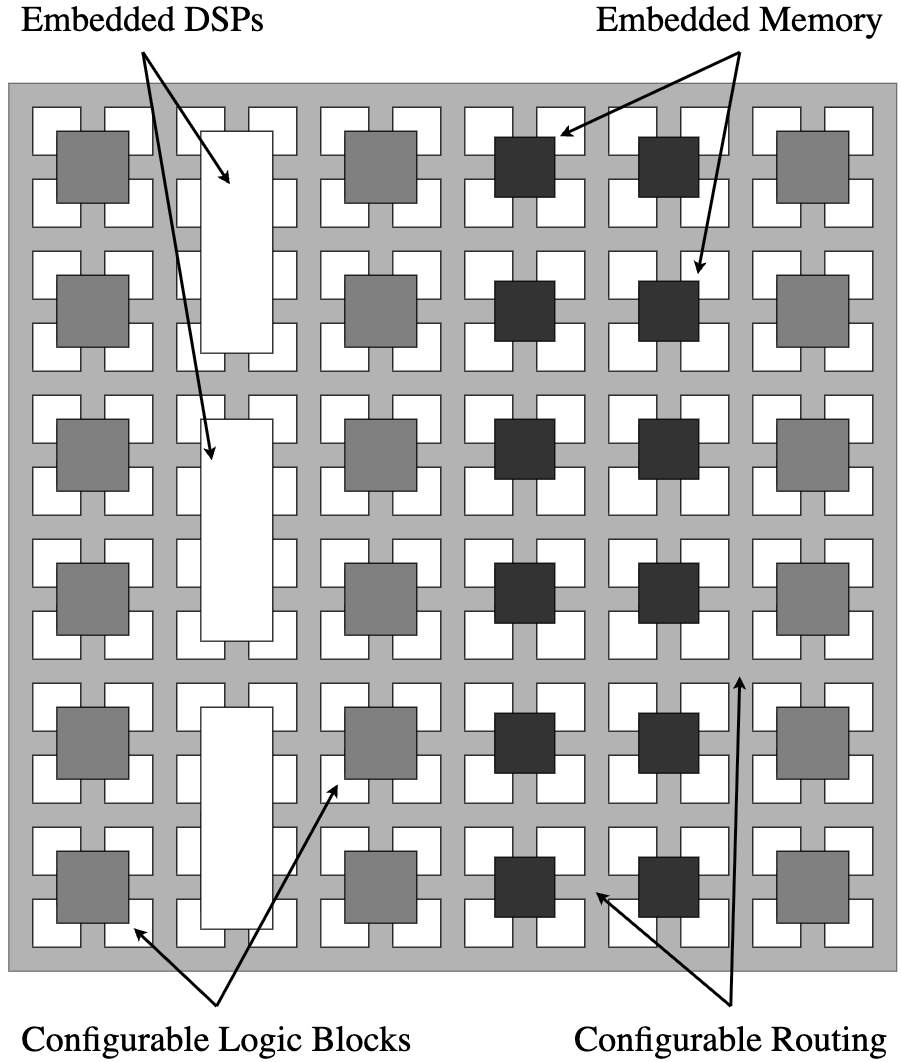
\includegraphics[width=0.55\textwidth]{figures/fpga.png}
	\end{center}
	\caption{}
	\label{fig:fpga}
\end{figure}
